\documentclass{article}
\usepackage[a4paper, margin=3cm]{geometry}
\usepackage{graphicx}
\usepackage{algorithm}
\usepackage{algpseudocode}
\usepackage{hyperref}
\usepackage{comment}
\usepackage{amsmath}
\usepackage{enumitem}
\usepackage{amsfonts}
\usepackage{tikz}
\usetikzlibrary{arrows.meta,positioning,fit,calc}
\usepackage{rotating}

\newtheorem{theorem}{Theorem}[section]   % numbered per section
\newtheorem{lemma}[theorem]{Lemma}       % shares numbering with theorem
\newtheorem{corollary}[theorem]{Corollary}
\newtheorem{definition}[theorem]{Definition}
\usepackage{titling}

% Title formatting
\pretitle{\centering\LARGE\bfseries\vspace{0em}}
\posttitle{\par\vspace{1em}}

\preauthor{\centering\large}
\postauthor{\par\vspace{1em}}

\predate{\centering\small}
\postdate{\par}


\setlength{\parindent}{0pt} % no indend automatically everywhere

\title{Project Report\\Binary Heap and Dijkstra's Algorithm}
\author{
	\centering
	Josefine Lindmar
	Sonja Joost
}
\date{\today} % empty date



\begin{document}

\maketitle

\section{Introduction}
Explain high level idea, name all challenges addresed in the upcoming sections

\section{Binary Heap}
Array vs Tree

\section{Dijkstra's algorithm}
\textbf{Goal.} Formalize Dijkstra's algorithm over finite graphs and prove correctness, using a priority queue abstraction. Our Lean development lives in \texttt{Projects/Lindmar\_Joost/Dijkstra.lean}.\\

We represent the graph as a finite simple graph so vertices have decidable equality (exactly how we have seen it in the BinarySort examples in class). Distances use extended natural numbers (so an unknown distance can be “infinity”), called \texttt{ENat} in Lean. The algorithm state is just a pair: a distance map from vertices to these extended naturals (\(\texttt{dist} : V \to \mathbb{N}_\infty\)) and a binary-heap priority queue (\(\texttt{queue} : \texttt{BinaryHeap}\)). The heap exposes abstract operations (empty check, extract-min, decrease-priority, size) and the proofs only rely on their contracts. 

The algorithm is split up into three parts: 
\begin{itemize}
	\item Relaxation (Lean: \texttt{relaxNeighbors}) is a simple loop over the neighbors of a vertex u that updates each neighbor v by setting $dist(v)$ to the minimum of its current value and $dist(u)+1$, and it conceptually decreases v’s priority in the heap when that happens.
	\item The recursive core of Dijkstra (Lean: \texttt{dijkstra\_rec}) repeatedly extracts the current minimum u, relaxes u’s neighbors (updating the distance map and heap), and then recurses on the new state.
	\item The top-level function (Lean: \texttt{dijkstra}) initializes distances with 0 at the source and infinity elsewhere, inserts the source into the heap, and starts the recursion.
\end{itemize}



\subsection*{Termination}
We split the implementation into three parts: \texttt{dijkstra} (a non-recursive wrapper), \texttt{dijkstra\_rec} (the recursive core), and \texttt{relaxNeighbors} (implemented as a fold over the finite list of neighbors). Hence termination needs to be shown only for \texttt{dijkstra\_rec}: \texttt{dijkstra} is trivially terminating because it does not recurse, and \texttt{relaxNeighbors} terminates by structural recursion on a finite list (Lean accepts it as a terminating fold), so no additional termination proof is required for them.

We prove termination by the measure \texttt{queue.sizeOf}: if \texttt{queue.isEmpty} the recursion stops, otherwise extracting the minimum yields \texttt{(u, queue')} and \texttt{BinaryHeap.sizeOf\_extract\_min\_lt\_of\_isEmpty\_eq\_false} gives \(\texttt{queue'.sizeOf} < \texttt{queue.sizeOf}\); since \texttt{relaxNeighbors} does not increase the heap size the post-relax queue has strictly smaller size than the original, so the \texttt{queue.sizeOf} measure decreases on every recursive call. In Lean this is written as \texttt{termination\_by queue.sizeOf} and discharged by applying \texttt{BinaryHeap.sizeOf\_extract\_min\_lt\_of\_isEmpty\_eq\_false} plus the trivial bookkeeping to turn the hypothesis into the expected \texttt{isEmpty = false} form.


\subsection*{Correcntess proof (\texorpdfstring{$\texttt{dijkstra\_correctness}$}{dijkstra\_correctness})}
\emph{Statement.} For any vertex \(v\), the algorithm’s output equals the graph distance $\delta$: \((\texttt{dijkstra}\ g\ s\ v)\ v = \delta(g,s,v)\).

The proof proceeds by fixing the algorithm's output and deriving a contradiction from any alleged disagreement with the true graph distance. Concretely, set
\[
\texttt{dist} := \texttt{dijkstra}\ g\ s\ v
\]
(in Lean: \texttt{set dist := (dijkstra g s v) with hdist}). First establish the global lower bound
\[
\forall u,\ \delta(s,u)\le \texttt{dist}\ u,
\]
provided by the lemma \texttt{neverUnderestimates}. Note also that \(\delta(s,s)=0\) and by \texttt{dijkstra\_source\_zero} the algorithm assigns \(0\) to the source, so any counterexample cannot be the source.

Assume, for contradiction, that there exists a vertex \(u\) with \(\texttt{dist}\ u \ne \delta(s,u)\). Choose such a \(u\) that minimizes \(\delta(s,u)\) (Lean: \texttt{minimalCounterexample}). By the previous remark we have \(\delta(s,u)>0\), so take a shortest path from \(s\) to \(u\); this yields a predecessor \(y\) with \(y\sim u\) and
\[
\delta(s,u)=\delta(s,y)+1
\]
(Lean: \texttt{existsPredOnShortestPath}). By minimality of \(u\) we have \(\delta(s,y)<\delta(s,u)\), hence \(\texttt{dist}\ y=\delta(s,y)\).

Now apply the algorithmic per-edge final bound \texttt{relaxAdj\_final\_bound} to the edge \(y\sim u\). That lemma (which internally uses \texttt{exists\_extract\_or\_top}, \texttt{relaxNeighbors\_adj\_upper}, and the \(y\)-stability lemmas such as \texttt{extracted\_value\_is\_final\_lemma}) yields
\[
\texttt{dist}\ u \le \texttt{dist}\ y + 1.
\]
Substituting \(\texttt{dist}\ y=\delta(s,y)\) and \(\delta(s,y)+1=\delta(s,u)\) gives \(\texttt{dist}\ u \le \delta(s,u)\). Together with the global lower bound \(\delta(s,u)\le \texttt{dist}\ u\) this forces equality \(\texttt{dist}\ u = \delta(s,u)\), contradicting the choice of \(u\).

Hence no counterexample exists, and we conclude \texttt{dijkstra\_correctness}: for every vertex \(v\) the algorithm's output equals the graph distance \(\delta(g,s,v)\).
\paragraph{Preconditions and placeholders.}
The development assumes the standard BinaryHeap contracts and builds the correctness proof from a number of named lemmas, many of which in turn rely on smaller auxiliary facts. Figure~\ref{fig:dijkstra-deps} illustrates the dependency relation between the main lemmas used in this file; For space and clarity some minor lemmas are not shown in the diagram. 

All of the lemmas have been fully formalized except for the search lemma \texttt{exists\_extract\_or\_top}, which is currently left as a \texttt{sorry}, and the lower bound leamm \texttt{neverUnderestimates}. A discussion of why those particular proof remain unfinished appears in the "Reflection on Efforts" section at the end of the report.

\begin{sidewaysfigure}
\centering
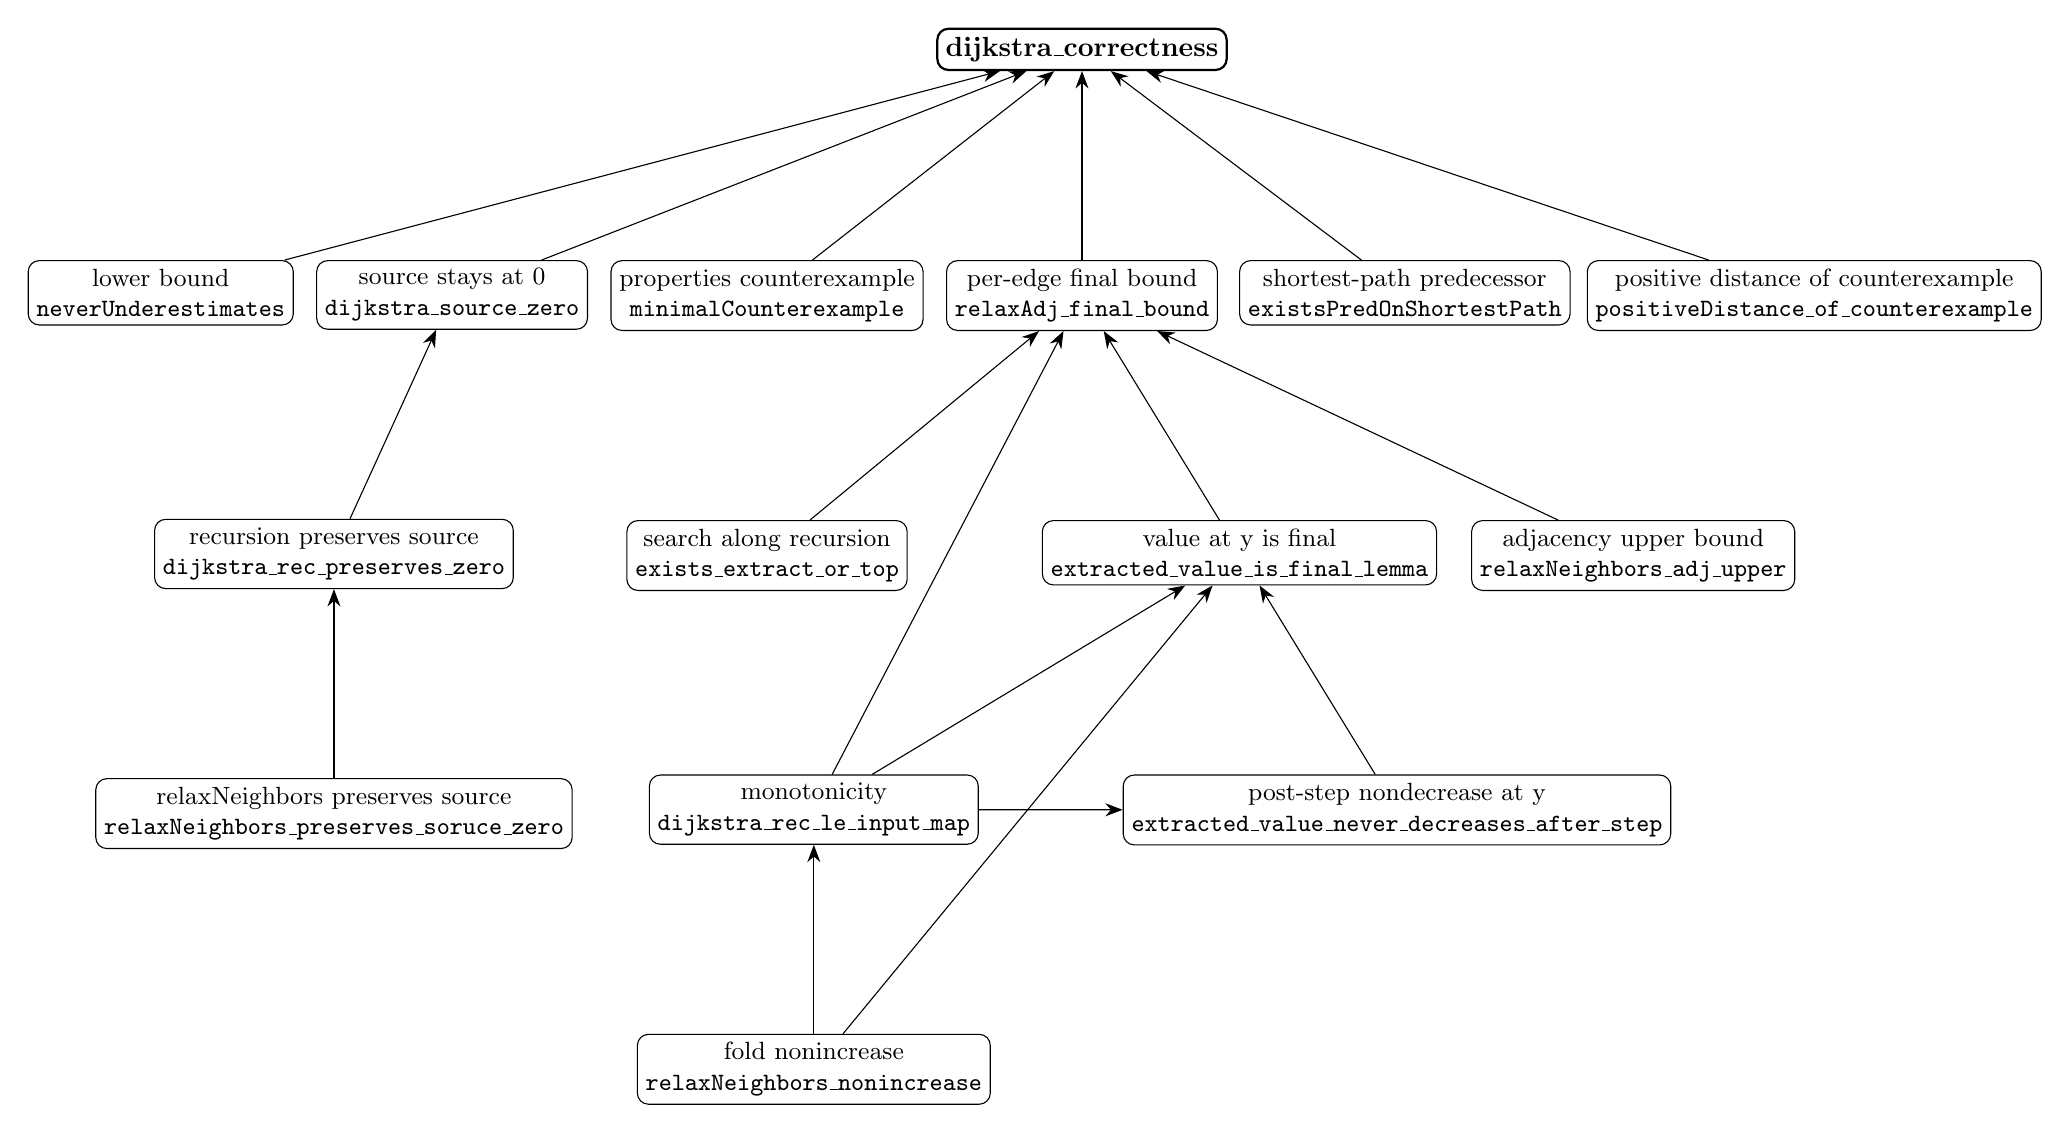
\begin{tikzpicture}[
  node distance=10mm and 12mm,
  box/.style={rectangle, draw, rounded corners, align=center, inner sep=3pt, font=\small},
  grp/.style={draw, rounded corners, inner sep=4pt, dashed},
  >={Stealth[length=2.2mm]},
  every edge/.style={draw, -{Stealth[length=2.2mm]}}
]
% Top layer: correctness
\node[box, font=\normalsize, thick] (CORR) {\textbf{dijkstra\_correctness}};

\node[box, below=24mm of CORR, xshift=-117mm] (LOWER) {lower bound\\\texttt{neverUnderestimates}};
\node[box, below=24mm of CORR, xshift=-80mm] (ZERO_TOP) {source stays at 0\\\texttt{dijkstra\_source\_zero}};
\node[box, below=24mm of CORR, xshift=-40mm] (CNT) {properties counterexample\\\texttt{minimalCounterexample}};
\node[box, below=24mm of CORR, xshift=0mm] (EDGE) {per-edge final bound\\\texttt{relaxAdj\_final\_bound}};
\node[box, below=24mm of CORR, xshift=41mm] (PRED) {shortest-path predecessor\\\texttt{existsPredOnShortestPath}};
\node[box, below=24mm of CORR, xshift=93mm] (CNT_DIST) {positive distance of counterexample\\\texttt{positiveDistance\_of\_counterexample}};

% Edges: correctness
\path (LOWER) edge (CORR);
\path (CNT) edge (CORR);
\path (ZERO_TOP) edge (CORR);
\path (CNT_DIST) edge (CORR);
\path (PRED) edge (CORR);
\path (EDGE) edge (CORR);

% LEVEL 2 (wider spacing to avoid horizontal overlap)
\node[box, below=24mm of EDGE, xshift=-40mm] (SEARCH) {search along recursion\\\texttt{exists\_extract\_or\_top}};
\node[box, below=24mm of EDGE, xshift=20mm]   (EVF)    {value at y is final\\\texttt{extracted\_value\_is\_final\_lemma}};
\node[box, below=24mm of EDGE, xshift=70mm]  (RAU)    {adjacency upper bound\\\texttt{relaxNeighbors\_adj\_upper}};
% Edges toward EDGE (per-edge final bound)
\path (SEARCH) edge (EDGE);
\path (EVF) edge (EDGE);
\path (RAU) edge (EDGE);

\node[box, below = 24mm of ZERO_TOP, xshift=-15mm] (ZERO_MIDDLE) {recursion preserves source\\\texttt{dijkstra\_rec\_preserves\_zero}};
\path (ZERO_MIDDLE) edge (ZERO_TOP);


% LEVEL 3
\node[box, below left=24mm and 8mm of EVF] (MONO) {monotonicity\\\texttt{dijkstra\_rec\_le\_input\_map}};
\node[box, below=24mm of EVF, xshift=20mm] (EVND) {post-step nondecrease at y\\\texttt{extracted\_value\_never\_decreases\_after\_step}};
\path (MONO) edge (EVF);
\path (MONO) edge (EDGE);
\path (MONO) edge (EVND);
\path (EVND) edge (EVF);

\node[box, below = 24mm of ZERO_MIDDLE] (ZERO_BOTTOM) {relaxNeighbors preserves source\\\texttt{relaxNeighbors\_preserves\_soruce\_zero}};
\path (ZERO_BOTTOM) edge (ZERO_MIDDLE);

% LEVEL 4
\node[box, below=24mm of MONO] (RNI) {fold nonincrease\\\texttt{relaxNeighbors\_nonincrease}};
\path (RNI) edge (MONO);
\path (RNI) edge (EVF);







% Group annotations (optional dashed boxes)
%\node[grp, fit=(RNI) (RAU), label={[align=center]below:{\footnotesize Relaxation facts}}] {};
%\node[grp, fit= (EVND) (EVF), label={[align=center]right:{\footnotesize Stability at $y$}}] {};

\end{tikzpicture}
\caption{Lemma dependency graph shaping the proof of correctness.}
\label{fig:dijkstra-deps}
\end{sidewaysfigure}

\newpage

\subsection*{Monotonicity of the recursion}
\emph{Statement.} Distances never increase along the recursion:
\[ (\texttt{dijkstra\_rec}\ g\ s\ t\ \texttt{dist}\ \texttt{queue})\ x \le \texttt{dist}\ x. \]
\emph{English proof.} By strong induction on \(\mathrm{sizeOf}(\texttt{queue})\). If empty, the result is \(\texttt{dist}\). Otherwise, after one step we recurse on a strictly smaller heap to obtain \(\texttt{dist}'\ x \le \texttt{dist}\ x\) using the IH and the fact that \texttt{relaxNeighbors} is pointwise nonincreasing.

\emph{Lean mapping.}
- Lemma \texttt{dijkstra\_rec\_le\_input\_map}: generalize the size to \(n\), revert state, apply \texttt{Nat.strong\_induction\_on}, split on \texttt{isEmpty}, perform one step with named equations (\texttt{step}, \texttt{u}, \texttt{queue'}, \texttt{next}), use size lemmas to apply the IH, then compose with \texttt{relaxNeighbors\_nonincrease}.

\subsection*{Properties of relaxation}
\emph{Pointwise nonincrease.} Folding does not increase any coordinate, since each step either keeps a value or lowers it. \emph{Lean:} \texttt{relaxNeighbors\_nonincrease}, proved by induction on the neighbor list.

\emph{Edge-wise upper bound.} If \(y\sim u\), then after relaxing neighbors of \(y\) once, the tentative value at \(u\) is at most \(\texttt{dist}\ y + 1\). \emph{Lean:} \texttt{relaxNeighbors\_adj\_upper}, proved by list induction plus membership of \(u\) in the neighbor list.

\subsection*{Extraction stability at a vertex}
\emph{Idea.} Once \(y\) is extracted, its value equals the value immediately after relaxing its neighbors and never decreases later. This captures Dijkstra's ``finalization'' of a node.

\emph{Lean mapping.}
- \texttt{MinGeYInvariant y (dist,queue)}: next extracted key \(\ge dist\ y\).
- \texttt{extracted\_value\_never\_decreases\_after\_step}: strong induction on the post-step heap size; the motive carries the invariant from \texttt{hInvPreserve}. Concludes \(\texttt{next}.1\ y \le (\texttt{dijkstra\_rec}\ g\ s\ t\ \texttt{next}.1\ \texttt{next}.2)\ y\).
- \texttt{extracted\_value\_is\_final\_lemma}: combine monotonicity (\( (\cdot)\ y \le \texttt{dist}\ y\)), preservation of \(y\) during relaxation (\(\texttt{next}.1\ y = \texttt{dist}\ y\)), and the previous lemma to get equality at \(y\).

\subsection*{Search along the recursion: extract-or-top}
\emph{Statement.} Either the final value at \(y\) is \(\top\), or there is a recursion state where the next extraction is \(y\) and one step of \texttt{dijkstra\_rec} is definitionally equal to continuing from \(\mathrm{relaxNeighbors}\ g\ y\ \cdot\ \cdot\).

\emph{English proof.} Run strong induction on the heap size while keeping the concrete state in scope. If the queue is empty then the final value at \(y\) is whatever sits in \(\texttt{dist}\) (in particular possibly \(\top\)). Otherwise, perform one step: if the extracted vertex is \(y\) we found the desired predecessor state; if not, recurse on the strictly smaller post-step heap until either \(y\) is extracted or the final is \(\top\).

\emph{Lean mapping.} Lemma \texttt{exists\_extract\_or\_top} (in progress): the induction predicate quantifies over all \(\texttt{dist},\texttt{q}\) with a size bound, and the step uses named equalities for \texttt{extract\_min} and \texttt{relaxNeighbors} so the one-step equality follows by definitional \texttt{simp}.

\subsection*{Final edge bound in the output map}
\emph{Statement.} For any edge \(y\sim u\), the output satisfies
\[ (\texttt{dijkstra}\ g\ s\ t)\ u \le (\texttt{dijkstra}\ g\ s\ t)\ y + 1. \]
\emph{English proof.} Use the extract-or-top dichotomy for \(y\). If the final value at \(y\) is \(\top\), the inequality holds trivially. Otherwise, identify the first state extracting \(y\); at that step, the relaxation at \(y\) ensures the post-step tentative value at \(u\) is \(\le (\texttt{dist}\ y + 1)\). Stability of \(y\) then transports this bound to the final output.

\emph{Lean mapping.} Lemma \texttt{relaxAdj\_final\_bound}: case-split on the search lemma, apply \texttt{relaxNeighbors\_adj\_upper} at the predecessor state, use \texttt{extracted\_value\_is\_final\_lemma} and monotonicity to lift it to the final map.

\subsection*{Global correctness (plan)}
\emph{Never underestimates.} Show \(\delta(s,u)\le (\texttt{dijkstra}\ g\ s\ t)\ u\) by induction on shortest paths (lemma \texttt{neverUnderestimates}).

\emph{Shortest-path predecessor.} For \(u\) with \(\delta(s,u)>0\), there exists \(y\) with \(y\sim u\) and \(\delta(s,u) = \delta(s,y)+1\) (lemma \texttt{existsPredOnShortestPath}), using Mathlib walks and minimality.

\emph{Minimal counterexample.} Assume a counterexample \(v\), pick minimal \(u\). Use the predecessor \(y\), its correctness by minimality, and the edge bound to get an upper bound \((\texttt{dijkstra}\ g\ s\ v)\ u\le \delta(s,u)\). Combined with the lower bound, obtain equality, contradiction (theorem \texttt{dijkstra\_correctness}).

\subsection*{English–Lean correspondence (by lemma)}
- \textbf{Algorithm/core:} \texttt{dijkstra\_rec}, \texttt{dijkstra}
- \textbf{Relaxation primitives:} \texttt{relaxNeighbors}, \texttt{relaxNeighbors\_nonincrease}, \texttt{sizeOf\_relaxNeighbors\_le}
- \textbf{Heap size laws:} \texttt{sizeOf\_extract\_min\_lt\_of\_isEmpty\_eq\_false}
- \textbf{Local invariant + stability:} \texttt{MinGeYInvariant}, \texttt{extracted\_value\_never\_decreases\_after\_step}, \texttt{extracted\_value\_is\_final\_lemma}
- \textbf{Search lemma:} \texttt{exists\_extract\_or\_top} (with strong induction on heap size)
- \textbf{Per-edge bound and finish:} \texttt{relaxNeighbors\_adj\_upper}, \texttt{relaxAdj\_final\_bound}, \texttt{neverUnderestimates}, \texttt{existsPredOnShortestPath}, \texttt{dijkstra\_correctness}

\subsection*{Open obligations still to discharge}
- Implement and verify the concrete heap operations and their size laws.
- Complete list-based inductive sublemmas inside \texttt{relaxNeighbors}.
- Finish the remaining induction engineering in the search lemma and stabilize the few marked \texttt{sorry}/\texttt{admit}.

\subsection*{Proof walkthrough and dependencies}
\emph{How the theorems interact.} Below we list the main lemmas, the direction they prove, and what they need.

- \textbf{Termination of recursion} (in \texttt{dijkstra\_rec}). Needs: heap facts
	\(\mathrm{sizeOf}(\mathrm{extract\_min}(q).2) < \mathrm{sizeOf}(q)\),
	\(\mathrm{sizeOf}(\mathrm{relaxNeighbors}(\cdot).2) \le \mathrm{sizeOf}(\cdot)\). Used by every strong-induction proof on the queue size.

- \textbf{Monotonicity} (\texttt{dijkstra\_rec\_le\_input\_map}). Needs: \texttt{relaxNeighbors\_nonincrease}. Used by stability at \(y\) (to get one side of equality) and in edge-bound lifting.

- \textbf{Relaxation properties}. Two pieces: (i) \texttt{relaxNeighbors\_nonincrease} (fold lemma), (ii) \texttt{relaxNeighbors\_adj\_upper} (single-step bound at an adjacent \(u\)). Used in the per-edge bound.

- \textbf{Local invariant and stability at y}. The invariant \texttt{MinGeYInvariant} is preserved between steps (assumed via \texttt{hInvPreserve}). Then
		exttt{extracted\_value\_never\_decreases\_after\_step} (strong induction on post-step heap) +
		exttt{extracted\_value\_is\_final\_lemma} yield that \(y\)'s value is fixed immediately after relaxing its neighbors. Used to propagate local bounds to the final map.

- \textbf{Search lemma} (\texttt{exists\_extract\_or\_top}). Needs: strong induction over queue size with a predicate that keeps the concrete state visible; uses definitional equalities of a single recursion step to connect states. Used by \texttt{relaxAdj\_final\_bound} to jump to the step where \(y\) is handled.

- \textbf{Per-edge final bound} (\texttt{relaxAdj\_final\_bound}). Needs: \texttt{exists\_extract\_or\_top}, \texttt{relaxNeighbors\_adj\_upper}, and the \(y\)-stability lemmas. Used directly in correctness.

- \textbf{Graph-theoretic path lemmas}. \texttt{existsPredOnShortestPath} (predecessor \(y\) on a shortest path) from Mathlib walk reasoning; independent of the heap proofs. Used in correctness to relate \(\delta(s,u)\) and \(\delta(s,y)\).

- \textbf{Lower bound} (\texttt{neverUnderestimates}). Needs only graph reasoning and the algorithm’s relaxation monotonicity; used in correctness to bound the output from below by true distance.

\paragraph{Dependency summary.}
\begin{itemize}[nosep]
	\item Termination facts \(\to\) strong induction on heap size.
	\item Fold lemmas \(\to\) monotonicity and single-step adjacency bound.
	\item Invariant + strong IH on post-step heap \(\to\) stability of \(y\).
	\item Search lemma + stability + adjacency bound \(\to\) per-edge final bound.
	\item Predecessor on shortest path + per-edge bound + lower bound \(\to\) correctness.
\end{itemize}




\section{Reflection on Efforts}
Task: "Describe the main challenges, one design decision you would reconsider, and what you learned about formalization."

Leave out: Challenges for Binary Heap 

Challenges for Dijkstra: 
- automation failed really often with maximum recursion depth reached 
- induction setup was hard, finding out the syntax to get the correct induction hypothesis, one time i could not figure it out to the end (theorem exists\_extract\_or\_top)
- i had to figure out the theorems needed with their proofs itself. we only found a super high level proof. all details i had to find out on my own

\section{Reflection on LLM Usage}

\begin{thebibliography}{9}
\bibitem{dijkstra}
Wikipedia,
\textit{Dijkstra's algorithm.} \url{https://en.wikipedia.org/wiki/Dijkstra%27s_algorithm}.

\bibitem{mathlib4}
Lean4, Mathlib4,
\textit{SimpleGraph documentation.} \url{https://leanprover-community.github.io/mathlib4_docs/Mathlib/Combinatorics/SimpleGraph/Basic.html#SimpleGraph}.

\bibitem{clrs}
Thomas H. Cormen, Charles E. Leiserson, Ronald L. Rivest, and Clifford Stein,  
\textit{Introduction to Algorithms},  
3rd edition,  
MIT Press, Cambridge, MA, 2009.
\end{thebibliography}

\end{document}
